\section{Bias-Variance Trade-Off}\label{sec:biasvar}

\subsection{Дилемма смещения-разброса}

Мы обсудили два вида бэкапов, доступных в model-free обучении: Монте-Карло бэкап и Temporal-Difference бэкап. На самом деле, они очень похожи, поскольку делают обновление вида
\begin{equation}\label{generalTD}
Q^\pi_{k+1}(s, a) \leftarrow Q^{\pi}_k(s, a) + \alpha_k \left( y_Q - Q^{\pi}_k(s, a) \right),
\end{equation}
и отличаются лишь выбором $y_Q$: Монте-Карло берёт reward-to-go, а TD-backup --- одношаговую бутстрапированную оценку с использованием уже имеющейся аппроксимации Q-функции.

Какой из этих двух вариантов лучше? Мы уже обсуждали недостатки Монте-Карло оценок: высокая дисперсия, необходимость играть до конца эпизодов, игнорирование структуры получаемой награды и потеря информации о соединениях состояний. Но не то, чтобы одношаговые оценки сильно лучше: на самом деле, они обладают полностью противоположными свойствами и проблемами. 

Да, одношаговые оценки аппроксимируют решение одношаговых уравнений Беллмана и приближают алгоритм динамического программирования: поэтому они не теряют информации о том, на каком шаге какой сигнал от среды был получен, и сохраняют информацию о сэмплах $s'$ из функции переходов; в том числе, как мы видели, одношаговые алгоритмы могут использовать реплей буфер, по сути и хранящий собранную выборку таких сэмплов. Взамен в одношаговых алгоритмах возникает проблема распространения сигнала.

\begin{example}
Представьте, что за 100 шагов вы можете добраться до сыра (+1). Пока вы не добьётесь успеха, сигнала нет, и ваша аппроксимация Q-функции остаётся всюду нулём. Допустим, вы учитесь с одношаговых оценок с онлайн опыта. После первого успеха +1 распространится лишь в пару $s, a$, непосредственно предшествующей получению сыра; после второго успеха +1 распространится из пары $s, a$ в предыдущую и так далее. Итого, чтобы распространить сигнал на 100 шагов, понадобится сделать 100 обновлений. С другой стороны, если бы использовалась Монте-Карло оценка, после первого же успеха +1 распространился бы во все пары $s, a$ из успешной траектории.
\end{example}

Вместо высокой дисперсии Монте-Карло оценок в одношаговых оценках нас ждёт большое \emph{смещение} (bias): если $y_Q$ оценено через нашу же текущую аппроксимацию через бутстрапирование, то оно не является несмещённой оценкой искомой $Q^{\pi}(s, a)$ и может быть сколь угодно <<неправильным>>. Как мы увидели, гарантии сходимости остаются, но естественно, что методы стохастической аппроксимации из-за смещения будут сходиться сильно дольше экспоненциального сглаживания, которому на вход поступают несмещённые оценки искомой величины. Но дисперсия $y_Q$ в temporal difference обновлениях, например, в алгоритме Q-learning \ref{alg:qlearning}, конечно, сильно меньше дисперсии Монте-Карло оценок: внутри нашей аппроксимации Q-функции уже усреднены все будущие награды, то есть <<взяты>> все интегралы, относящиеся к будущим после первого шага наградам. Итого одношаговая оценка $y_Q$ --- случайная величина только от $s'$, а не от всего хвоста траектории $s', a', s'' \dots$. Выбор между оценками с высокой дисперсией и отсутствием смещения (Монте-Карло) и оценками с низкой дисперсией и большим смещением (одношаговые оценки) --- особая задача обучения с подкреплением, называемая \emph{bias-variance trade-off}.

\subsection{N-step Temporal Difference}

Какие есть промежуточные варианты между одношаговыми оценками и Монте-Карло оценками? Давайте заглядывать в будущее не на один шаг и не до самого конца, а на $N$ шагов. Итак, пусть у нас есть целый фрагмент траектории:

\begin{definition}
Фрагмент траектории $s, a, r, s', a', r', s'', a'', r'', \dots s^{(N)}, a^{(N)}$, где $s^{(N)}, a^{(N)}$  --- пара состояние-действие, встретившаяся через $N$ шагов после оцениваемой пары $s, a$, будем называть \emph{роллаутом} (rollout) длины $N$.
\end{definition}

\begin{definition}
\emph{$N$-шаговой оценкой} (N-step estimation) для $Q^{\pi}(s, a)$ назовём следующий таргет:
$$y_Q \coloneqq r + \gamma r' + \gamma^2 r'' + \dots + \gamma^{N-1} r^{(N-1)} + \gamma^N Q^{\pi}(s^{(N)}, a^{(N)}),$$
\end{definition}

Такой таргет является стохастической аппроксимацией правой части $N$-шагового уравнения Беллмана \eqref{NstepBellman}, и формула \eqref{generalTD} с таким таргетом позволяет эту систему уравнений решать в model-free режиме. По каким переменным мы заменили интегралы на Монте-Карло приближения в такой оценке? По переменным $s', a', s'', a'' \dots s^{(N)}, a^{(N)}$, которые, пусть и не все присутствуют явно в формуле, но неявно задают то уравнение, которое мы решаем. Соответственно, чтобы выучить $Q^{\pi}(s, a)$, нужно, чтобы состояния приходили из функции переходов, а действия --- из оцениваемой стратегии $\pi$. Другими словами, роллаут, использованный для построения таргета, должен быть порождён оцениваемой стратегией.

Сразу заметим, что при $N \HM> 1$ нам необходимо иметь в этой оценке $a' \HM\sim \pi(a \HM\mid s), s'' \HM\sim p(s'' \mid s', a')$. Это означает, что мы не можем получить такую оценку с буфера: действительно, в буфере для данной четвёрки $s, a, r, s'$ не лежит сэмпл $a' \HM\sim \pi(a \HM\mid s)$, ведь в произвольном буфере $a'$ генерируется стратегией сбора данных (старой версией стратегией или <<экспертом>>). Само по себе это, вообще говоря, не беда: мы могли бы взять из буфера четвёрку, прогнать стратегию $\pi$, которую хотим оценить, на $s'$ и сгенерировать себе сэмпл $a'$; но для него мы не сможем получить сэмпл $s''$ из функции переходов! Поэтому обучаться на многошаговые оценки с буфера не выйдет; по крайней мере, без какой-либо коррекции.

Почему гиперпараметр $N$ отвечает за bias-variance trade-off? Понятно, что при $N \HM\to \infty$ оценка переходит в Монте-Карло оценку. С увеличением $N$ всё больше интегралов заменяется на Монте-Карло оценки и растёт дисперсия; наше же смещённое приближение будущих наград $Q^{\pi}(s^{(N)}, a^{(N)})$, которое может быть сколь угодно неверным, домножается на $\gamma^N$, и во столько же раз сбивается потенциальное смещение; с ростом $N$ оно уходит в ноль. Замешивая в оценку слагаемое $r + \gamma r' + \gamma^2 r'' + \dots + \gamma^{N-1} r^{(N-1)}$ мы теряем информацию о том, что из этого в какой момент было получено, но и начинаем распространять сигнал в $N$ раз <<быстрее>> одношаговой оценки.

Для удобства дальнейшего повествования введём следующие обозначения. Пусть мы взаимодействуем в среде при помощи стратегии $\pi$, которую хотим оценить; также будем считать learning rate $\alpha$ константным. 
\begin{definition}
Введём такое обозначение \emph{$N$-шаговой временной разности} (N-step temporal difference) для пары $s, a$:
\begin{equation*}
\Psi_{(N)} (s, a) \coloneqq \sum_{t=0}^{N-1} \gamma^{t} r^{(t)} + \gamma^N Q^\pi(s^{(N)}, a^{(N)}) - Q^\pi(s, a)
\end{equation*}
где $Q^{\pi}$ --- текущая аппроксимация Q-функции, $s, a, \dots s^{(N)}, a^{(N)}$ --- роллаут, порождённый $\pi$.
\end{definition}

Ранее мы обсуждали temporal difference, в котором мы сдвигали нашу аппроксимацию на $\Psi_{(1)}(s, a)$:
\begin{align*}
Q^{\pi}(s, a) &\leftarrow Q^{\pi}(s, a) + \alpha (r(s, a) + \gamma Q^{\pi}(s', a') - Q^{\pi}(s, a)) = \\ &= Q^{\pi}(s, a) + \alpha \Psi_{(1)}(s, a)
\end{align*}
Теперь же мы можем обобщить наш метод, заменив оценку Q-функции на многошаговую оценку:
$$Q^{\pi}(s, a) \leftarrow Q^{\pi}(s, a) + \alpha \Psi_{(N)}(s, a)$$

\needspace{5\baselineskip}
\begin{wrapfigure}{r}{0.35\textwidth}
%\vspace{-0.3cm}
\centering
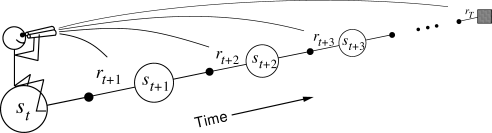
\includegraphics[width=0.35\textwidth]{Images/forward_view.png}
\vspace{-0.5cm}
\end{wrapfigure}
Естественно, для такой N-шаговой оценки нам нужно знать своё будущее на $N$ шагов вперёд (естественно), точно так же, как для Монте-Карло оценок нужно доигрывать эпизоды до конца. Такой взгляд на оценки называется <<\emph{forward view}>>: мы после выполнения $a$ из $s$ знаем <<вперёд>> своё будущее и можем обновить оценочную функцию для этой пары.

\subsection{Backward View}
Оказывается, мы можем посмотреть на задачу немного по-другому. Рассмотрим эту идею, развив пример с кафе \ref{ex:cafe}.

\begin{example}
Ещё раз сядем в кафе ($s$) и захотим вернуться домой. Текущая аппроксимация даёт $-Q^\pi(s, a) = 30$ минут. Делаем один шаг в среде: тратим одну минуту ($-r$) и обнаруживаем пробку ($s'$). Новая оценка времени возвращения даёт: $-Q^\pi(s', a') = 40$ минут, соответственно с нами случилась одношаговая временная разность $\Psi_{(1)}(s, a) = 41 - 30 \HM= 11$ минут, которая позволяет нам корректировать $Q^\pi(s, a)$.

\needspace{7\baselineskip}
\begin{wrapfigure}{r}{0.3\textwidth}
\vspace{-0.3cm}
\centering
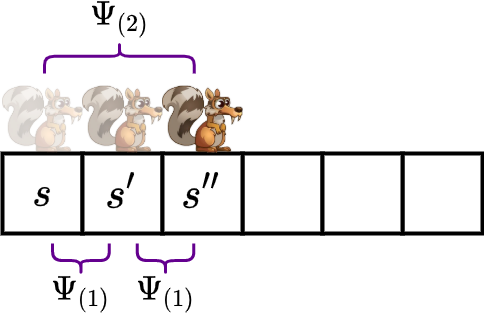
\includegraphics[width=0.3\textwidth]{Images/MultiStepErrors3.png}
\vspace{-0.3cm}
\end{wrapfigure}

Давайте сделаем ещё один шаг в среде: тратим одну минуту $-r'$, видим пожар $s''$ и получаем новую оценку $-Q^\pi(s'', a'') = 60$ минут. Тогда мы можем посчитать как одношаговую временную разность для пары $s', a'$, равную $\Psi_{(1)}(s', a') \HM= 61 \HM- 40 \HM= 21$ минуте, и уточнить свою аппроксимацию Q-функции для пробки; а можем посчитать и двухшаговую временную разность для кафе: мы потратили две минуты $r + r'$ на два шага и наша нынешнее приближение равно 60 минутам. Итого двухшаговая временная разность равна $\Psi_{(2)}(s, a) \HM= 62 - 30 = 32$ минуты. Forward view говорит следующее: если мы хотим учиться на двухшаговые оценки вместо одношаговых, то нам не следовало на первом шаге использовать 11 минут для обновления $Q^\pi(s, a)$, а нужно было дождаться второго шага, узнать двухшаговую ошибку в 32 минуты и воспользоваться ей.

Но понятно, что двухшаговая ошибка это сумма двух одношаговых ошибок! Наши 32 минуты ошибки --- это 11 минут ошибки после выхода из кафе в пробку плюс 21 минута ошибки от выхода из пробки в пожар. Давайте после первого шага используем уже известную часть ошибки в 11 минут, а на втором шаге, если мы готовы обучаться с двухшаговых ошибок, возьмём и добавим недостающие 21 минуту.
\end{example}

Формализуем эту идею. Это означает, что после совершения первого шага <<из кафе>> мы можем, зная $s, a, r, s', a'$ сразу же обновить нашу Q-функцию:
$$
Q^{\pi}(s, a) \leftarrow Q^{\pi}(s, a) + \alpha \Psi_{(1)}(s, a)
$$
Затем мы делаем ещё один шаг в среде, узнавая $r', s'', a''$ и временную разность за этот случившийся шаг $\Psi_{(1)}(s', a')$. Тогда мы можем просто ещё в нашу оценку Q-функции добавить слагаемое:
$$
Q^{\pi}(s, a) \leftarrow Q^{\pi}(s, a) + \alpha \gamma \Psi_{(1)}(s', a')
$$
Суммарное обновление Q-функции в силу \eqref{NstepAdvSimplified} получится эквивалентным двухшаговому обновлению:
$$
Q^{\pi}(s, a) \leftarrow Q^{\pi}(s, a) + \alpha (\Psi_{(1)}(s, a) + \gamma \Psi_{(1)}(s', a')) = Q^{\pi}(s, a) + \alpha \Psi_{(2)}(s, a)
$$

Понятно, что можно обобщить эту идею с двухшаговых ошибок на $N$-шаговые: действительно, ошибка за $N$ шагов равна сумме одношаговых ошибок за эти шаги.

\begin{theorem}\,
\begin{equation}\label{NstepAdvSimplified}
\Psi_{(N)}(s, a) = \sum_{t = 0}^{N - 1} \gamma^t \Psi_{(1)}(s^{(t)}, a^{(t)})
\end{equation}

\needspace{7\baselineskip}
\begin{wrapfigure}{r}{0.3\textwidth}
\vspace{-0.3cm}
\centering
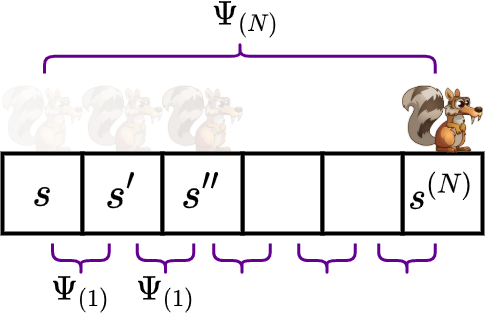
\includegraphics[width=0.3\textwidth]{Images/MultiStepErrors4.png}
\vspace{-0.3cm}
\end{wrapfigure}
\beginproof
Докажем по индукции. Для $N = 1$ справа стоит только одно слагаемое, $\Psi_{(1)}(s, a)$, то есть одношаговая оценка.

Пусть утверждение верно для $N$, докажем для $N + 1$. В правой части при увеличении $N$ на единицу появляется одно слагаемое, то есть для доказательства достаточно показать, что
$$\Psi_{(N + 1)}(s, a) = \Psi_{(N)}(s, a) + \gamma^N \Psi_{(1)}(s^{(N)}, a^{(N)}) = (*)$$
Убедимся в этом, подставив определения:
\begin{align*}
(*) &= \sum_{t = 0}^{N - 1}\gamma^t r^{(t)} + \gamma^N V^\pi(s^{(N)}) - V^\pi(s) + \gamma^N \left( r^{(N)} + \gamma V^\pi(s^{(N+1)}) - V^\pi(s^{(N)}) \right) = \\
&= \sum_{t = 0}^{N}\gamma^t r^{(t)} + \gamma^{N+1}V^\pi(s^{(N+1)}) - V^\pi(s) = \\
&= \Psi_{(N + 1)}(s, a)   \tagqed
\end{align*}
\end{theorem}

\needspace{7\baselineskip}
\begin{wrapfigure}{l}{0.35\textwidth}
\vspace{-0.3cm}
\centering
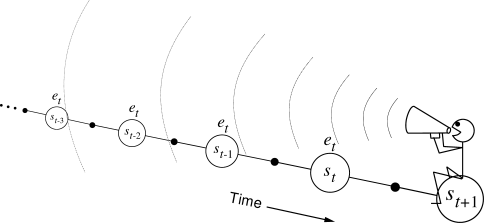
\includegraphics[width=0.35\textwidth]{Images/backward_view.png}
%\vspace{-0.3cm}
\end{wrapfigure}
Итого, оказывается, мы можем, на каждом шаге добавляя к оценкам Q-функции ранее встречавшихся в эпизоде парах $s, a$ только что случившуюся одношаговую ошибку $\Psi_{(1)}(s, a)$, получать $N$-шаговые обновления: достаточно пару $s, a$, посещённую $K$ шагов назад, обновить с весом $\alpha \gamma^K$. То есть мы начинаем действовать по-другому: зная, что было в прошлом, мы правильным образом обновляем оценочные функции пар $s, a$ из прошлого, используя только что случившуюся ошибку (<<настоящее>>). Такой подход к обновлению оценочной функции называется, соответственно, <<\emph{backward view}>>, и он даёт интересные возможности.

\subsection{Eligibility Trace}

Рассмотрим случай $N = +\infty$, то есть допустим, что мы готовы обновлять Q-функцию с reward-to-go. Наше рассуждение, можно сказать, позволяет теперь это делать, не доигрывая эпизоды до конца: мы сразу же в ходе эпизода можем уже <<начинать>> сдвигать Q-функцию в правильном направлении. Это позволяет запустить <<как бы Монте-Карло>> алгоритм даже в неэпизодичных средах. Однако, на каждом шаге нам нужно перебирать все встретившиеся ранее в эпизоде пары $s, a$, чтобы обновить их, и, если эпизоды длинные (или среда неэпизодична), это хранение истории на самом деле становится избыточным. 

Допустим, мы сделали шаг в среде и получили на этом одном шаге какую-то одношаговую ошибку $\Psi_{(1)}$. Рассмотрим какую-нибудь пару $s, a$. С каким весом, помимо learning rate, нужно добавить эту ошибку к нашей текущей аппроксимации? Эта пара в течение прошлого эпизода была, возможно, посещена несколько раз, и за каждое посещение вес увеличивается на $\gamma^K$, где $K$ --- число шагов с момента посещения.

\begin{definition}
Будем называть $e_t(s, a)$ \emph{следом} (eligibility trace) пары $s, a$ в момент времени $t$ эпизода число, проинициализированное нулём и далее определённое следующим образом:
$$e_t(s, a) \coloneqq \begin{cases}
\gamma e_{t - 1}(s, a) + 1 \quad & \text{если } s = s_t, a = a_t \\
\gamma e_{t - 1}(s, a) \quad & \text{иначе}
\end{cases}$$
\end{definition}

\needspace{7\baselineskip}
\begin{wrapfigure}{r}{0.35\textwidth}
\vspace{-0.8cm}
\centering
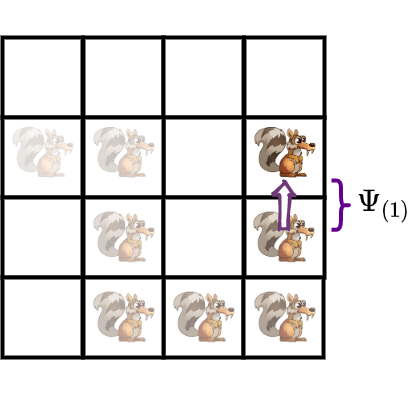
\includegraphics[width=0.3\textwidth]{Images/EligibilityTrace.png}
\vspace{-0.6cm}
\end{wrapfigure}

Итак, мы получили, что нам для Монте-Карло алгоритма вовсе не нужно хранить историю: мы можем просто хранить eligibility trace и на каждом шаге обновлять абсолютно все ячейки нашей таблицы: $\forall s, a \colon$
\begin{equation}\label{eligibilitytraceupdate}
    Q(s, a) \leftarrow Q(s, a) + \alpha e_t(s, a) \Psi_{(1)}(s_t, a_t),
\end{equation}
где $\Psi_{(1)}(s_t, a_t)$ --- одношаговая ошибка на шаге $t$. Если в ходе таких обновлений learning rate и оцениваемая стратегия не меняется, наши обновления в точности соответствуют Монте-Карло.

\subsection{TD($\lambda$)}

Заметим, что если мы хотим ограничиться лишь, допустим, одношаговыми, то мы можем использовать просто <<другое>> определение следа:
$$e_t(s, a) \coloneqq \begin{cases}
1 \quad & \text{если } s = s_t, a = a_t \\
0 \quad & \text{иначе}
\end{cases}$$
Иначе говоря, для одношаговых оценок нам нужно домножать след не на $\gamma$, а на ноль. Тогда вектор $e(s, a)$ на каждой итерации будет нулевым за исключением одной лишь только что встреченной пары $s_t, a_t$, для которой он будет равен единице, и обновление \ref{eligibilitytraceupdate} будет эквивалентно обычному одношаговому temporal difference.

\needspace{15\baselineskip}
\begin{wrapfigure}{r}{0.3\textwidth}
%\vspace{-0.5cm}
\centering
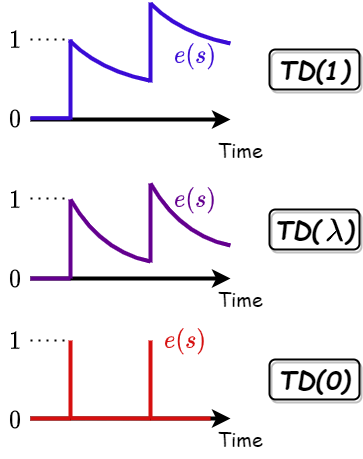
\includegraphics[width=0.3\textwidth]{Images/Traces.png}
\vspace{-1.5cm}
\end{wrapfigure}
Видно, что мы теперь можем придумать другой вид <<промежуточных оценок>> между Монте-Карло и одношаговыми. Давайте как-нибудь по-другому будем след <<затухать>>. Если на очередном моменте времени след для пар $s, a$ затухает сильнее, чем в $\gamma$ раз (например, в ноль), то мы лишь будем обращать больше внимания на ту оценку, которая уже замешана в обновлении $Q(s, a)$, и меньше внимания на оценки большей длины. Классический и хорошо исследованный способ это сделать --- ввести ещё один параметр, $\lambda \in [0, 1]$ --- <<коэффициент затухания>> --- и тушить след не с коэффициентом $\gamma$, а с коэффициентом $\gamma \lambda$.

Итак, мы получили алгоритм TD($\lambda$) оценивания стратегии, или temporal difference с параметром $\lambda$, который при $\lambda \HM= 1$ эквивалентен Монте-Карло алгоритму (с постоянным обновлением Q-функции <<по ходу эпизода>>), а при $\lambda \HM = 0$ эквивалентен одношаговому temporal difference методу, который мы, в частности, применяли в Q-learning и SARSA для оценивания стратегии.

\begin{algorithm}{TD($\lambda$)}
\textbf{Вход:} $\pi$ --- стратегия \\
\textbf{Гиперпараметры:} $\alpha$ --- параметр экспоненциального сглаживания, $\lambda \in [0, 1]$ --- степень затухания следа

\vspace{0.3cm}
Инициализируем $Q(s, a)$ произвольно для всех $s \in \St, a \in \A$ \\
Инициализируем $e(s, a)$ нулём для всех $s \in \St, a \in \A$ \\
Наблюдаем $s_0$, $a_0$ --- случайно \\
\textbf{На $k$-ом шаге:}
\begin{enumerate}
    \item играем $a_k$ и наблюдаем $r_k, s_{k+1}$
    \item выбираем $a_{k+1} \sim \pi(a_{k+1} \mid s_{k+1})$
    \item обновляем след $e(s_k, a_k) \leftarrow e(s_k, a_k) + 1$
    \item считаем одношаговую ошибку $\Psi_{(1)} \coloneqq r_k + \gamma Q(s_{k+1}, a_{k+1}) - Q(s_k, a_k)$
    \item для всех пар $s, a$ обновляем $Q(s, a) \leftarrow Q(s, a) + \alpha e(s, a) \Psi_{(1)}$
    \item для всех пар $s, a$ обновляем $e(s, a) \leftarrow \gamma \lambda e(s, a)$
\end{enumerate}

\vspace{0.3cm}
\textbf{Выход:} $Q(s, a)$
\end{algorithm}

Мы обсуждали и выписали этот алгоритм для Q-функции для задачи именно оценивания стратегии; естественно, мы могли бы сделать это для V-функции или добавить policy improvement после, например, каждого шага в среде, получив табличный алгоритм обучения стратегии. В таком алгоритме сохраняются гарантии сходимости.

Давайте подумаем, чему будет соответствовать случай $\lambda \in (0, 1)$. Тогда в течение эпизода мы обновляем ячейку Q-функции со следующим весом:
$$Q(s, a) \leftarrow Q(s, a) + \alpha \sum_{t \ge 0} (\gamma \lambda)^t \Psi_{(1)}(s^{(t)}, a^{(t)})$$

Очевидно, такое обновление не эквивалентно никаким $N$-шаговым temporal difference формулам: в нём замешана как Монте-Карло оценка, то есть замешана вся дальнейшая награда (весь будущий сигнал), так и одношаговая оценка: ведь понятно, что слагаемое $\gamma Q(s', a')$ не сократится с соответствующим слагаемым из $\Psi_{(1)}(s', a')$, как это было раньше, из-за домножения на $\lambda$, и с весом $1 - \lambda$ <<останется>> в итоговой формуле. Разберёмся, какой вклад даёт каждое слагаемое:

\begin{theoremBox}[label=th:tdlambda]{}\,
\begin{equation}\label{TDlambda}
\sum_{t \ge 0} \gamma^t \lambda^t \Psi_{(1)}(s^{(t)}, a^{(t)}) = (1 - \lambda) \sum_{t > 0} \lambda^{t-1} \Psi_{(t)}(s, a)
\end{equation}
\begin{proof} И справа, и слева в сумме стоит слагаемые двух видов: награды за шаг $r^{(t)}$ (для $t \ge 0$) и Q-оценки $Q(s^{(t)}, a^{(t)})$ с какими-то весами. Поймём, что они стоят с одними и теми же весами.

Справа награда за шаг $r^{(t)}$ участвует во всех слагаемых, начиная с $t + 1$-го, во всех них дисконтирована на $\gamma^t$ и входит в ансамбль с весом $(1 - \lambda)(\lambda^t + \lambda^{t+1} + \dots)$. Итого её вес --- $\gamma^t\lambda^t$. А слева эта награда входит только в одно слагаемое: в одношаговую оценку для $\Psi_{(1)}(s^{(t)}, a^{(t)})$, и с тем же весом.

Справа аппроксимация $Q(s^{(t)}, a^{(t)})$ при $t > 0$ входит только в одно слагаемое, в $\Psi_{(t)}(s, a)$, с весом $(1 - \lambda)\lambda^{t - 1}\gamma^t$. Слева $Q(s^{(t)}, a^{(t)})$ входит в два слагаемых: в $\Psi_{(1)}(s^{(t-1)}, a^{(t-1)})$ с положительным весом $\gamma^t\lambda^{t-1}$ и в $\Psi_{(1)}(s^{(t)}, a^{(t)})$ с отрицательным весом $-\gamma^t\lambda^t$. Сумма этих двух коэффициентов совпадает с $(1 - \lambda)\lambda^{t - 1}\gamma^t$.

Наконец, $-Q(s, a)$ входит справа во все слагаемые с суммарным весом $(1 - \lambda)(1 + \lambda + \lambda^2 + \dots) = 1$, а слева он присутствует только в $\Psi_{(1)}(s, a)$, тоже с весом 1.
\end{proof}
\end{theoremBox}

\needspace{5\baselineskip}
\begin{wrapfigure}{r}{0.4\textwidth}
\vspace{-0.3cm}
\centering
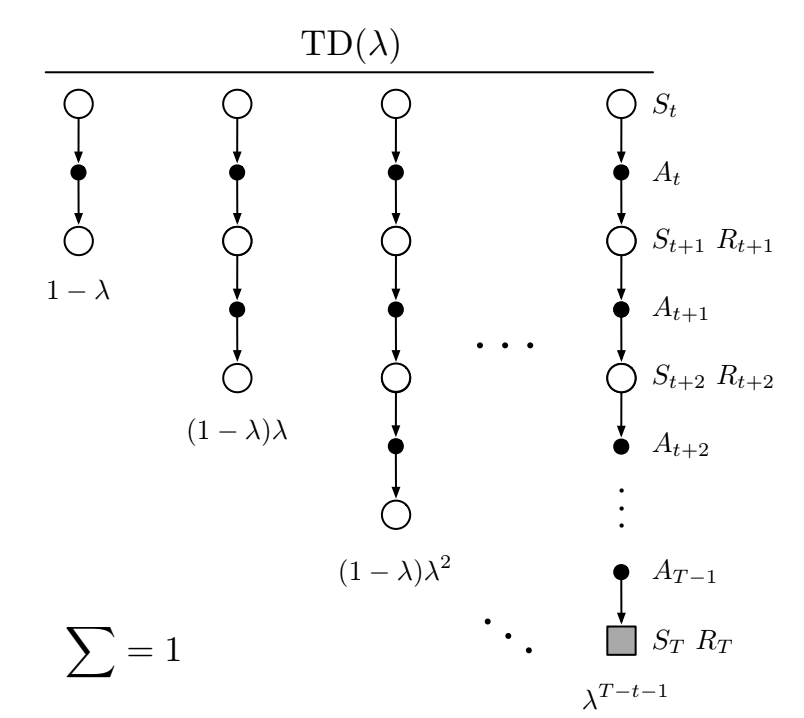
\includegraphics[width=0.4\textwidth]{Images/td_lambda.png}
\vspace{-0.7cm}
\end{wrapfigure}

Мы доказали, что TD($\lambda$) просто заансамблировал многошаговые оценки разной длины. Мы взяли одношаговую оценку с весом $\lambda$, двухшаговую с весом $\lambda^2$, $N$-шаговую с весом $\lambda^N$ и так далее. Сумма весов в ансамбле, как водится, должна равняться единице, отсюда в формуле домножение на $1 - \lambda$.

Если через $N$ шагов после оцениваемой пары $s, a$ эпизод закончился, то все многошаговые оценки длины больше $N$, понятно, совпадают с $N$-шаговой и равны reward-to-go. Следовательно, в такой ситуации reward-to-go по определению замешивается в оценку с весом $(1 - \lambda)(\lambda^{N-1} + \lambda^{N} + \dots) \HM= \lambda^{N-1}$.

Мы привыкли, что любая формула обновления для нас --- стохастическая аппроксимация решения какого-то уравнения. TD($\lambda$) не исключение. Если $N$-шаговая оценка направляет нас в сторону решения $N$-шагового уравнения Беллмана $Q^{\pi} \HM= \B^N Q^{\pi}$, то ансамбль из оценок направляет нас в сторону решения ансамбля $N$-шаговых уравнений Беллмана:
$$Q^{\pi} = (1 - \lambda)(\B Q^{\pi} + \lambda \B^2 Q^{\pi} + \lambda^2 \B^3 Q^{\pi} + \dots ) = (1 - \lambda) \sum_{N > 0} \lambda^{N-1} \B^N Q^{\pi}$$

Поскольку $Q^{\pi}$ является неподвижной точкой для операторов $\B^N$ для всех $N$, то и для их выпуклой комбинации, <<ансамбля>>, он тоже будет неподвижной точкой. Итого TD($\lambda$) дало нам прикольную идею: мы не могли выбрать одну из многошаговых оценок, и поэтому взяли их все сразу.

\begin{remark}
Полезность TD($\lambda$) в том, что $\lambda$ непрерывно и позволяет более гладкую настройку <<длины следа>>. При этом даже если $\lambda < 1$, в оценку <<поступает>> информация о далёкой награде.
\end{remark}